\documentclass[12pt,a4paper]{article}
\usepackage[utf8]{inputenc}
\usepackage[french]{babel}
\usepackage[T1]{fontenc}
\usepackage{amsmath}
\usepackage{amsfonts}
\usepackage{amssymb}
\usepackage{makeidx}
\usepackage{graphicx}
\usepackage{lmodern}
\usepackage{index}
%\usepackage{hyperref}
\newcommand{\HRule}{\rule{\linewidth}{0.5mm}}
%\usepackage{kpfonts}
\usepackage{fourier}
\usepackage[left=2cm,right=2cm,top=2cm,bottom=2cm]{geometry}
\author{Sarah Kaddah}
\title{Rapport de stage}

%%%%%%%%%%Interligne
\renewcommand{\baselinestretch}{1.5}
\begin{document}
%%%%%%%%%%%%%%%%%%%%%%%%%%%%%%%%%%%%%%%%%%%%%%%%%%%%%%%%%%%%%%%%%
%%%%%%%%%%%%%%%%%%%%%%1ere page%%%%%%%%%%%%%%%%%%%%%%%%%%%%%%%%%%
%%%%%%%%%%%%%%%%%%%%%%%%%%%%%%%%%%%%%%%%%%%%%%%%%%%%%%%%%%%%%%%%%
%%%%%%%%%%%%%%%%%%%%%%%%%%%%%%%%%%%%%%%%%%%%%%%%%%%%%%%%%%%%%%%%%
\begin{titlepage}
  \begin{sffamily}
  \begin{center}
	\large{Master 2 Biologie-Informatique/ Bioinformatique \hfill 2017-2018}
	\flushleft{\large{Université Paris Diderot - Paris 7}}
	
%	\begin{center}
%		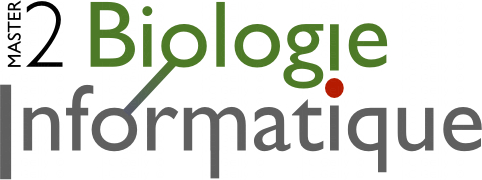
\includegraphics[scale=0.3]{img/m2.png} \hfill
%		
\includegraphics[scale=0.1]{img/p7.png}
%	\end{center}

\begin{tabular}{c}
\\ \\ \\
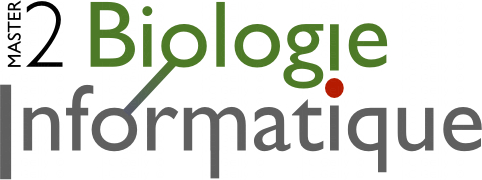
\includegraphics[scale=0.3]{img/m2.png}
\end{tabular}
\hfill
\begin{tabular}{c}
\\

\includegraphics[scale=0.1]{img/p7.png}
\end{tabular}

%%%%%%%%% Title    
    \HRule \\[0.2cm]
    { \huge \bfseries \center{Etude de la fonction et des mécanismes d'évolution des séquences répétées centromériques chez les Primates}\\[0.4cm] }
    \HRule \\[2cm]
%%%%%%%%Centre de la page    
\begin{center}\LARGE{\textbf{Sarah Kaddah}}\end{center}
\begin{center}\Large{Tuteur: Lo\"{i}c Ponger}\end{center}~\\[0.5cm]
%%%%%%%%% Bottom of the page
\center{\large{Structure et Instabilité des Génomes}}
\center{\large{ MNHN - CNRS UMR 7196 / INSERM U1154 - Sorbonne Universités}}\\[1cm]

%	\begin{center}
%		
\includegraphics[scale=0.2]{img/mnhn.jpg} \hfill
%		
\includegraphics[scale=0.08]{img/cnrs.png} \hfill
%		
\includegraphics[scale=0.08]{img/inserm.jpg}
%	\end{center} 

\begin{tabular}{cc}
 \hspace*{3cm} &  

\includegraphics[scale=0.2]{img/mnhn.jpg}
\end{tabular}
\hfill
\begin{tabular}{c}

\includegraphics[scale=0.08]{img/inserm.jpg}
\end{tabular}
\hfill
\begin{tabular}{cc}

\includegraphics[scale=0.08]{img/cnrs.png} &
\hspace*{3cm}
\end{tabular}

%%%%%%%%% END
  \end{center}
  \end{sffamily}
\end{titlepage}
%%%%%%%%%%%%%%%%%%%%%%%%%%%%%%%%%%%%%%%%%%%%%%%%%%%%%%%%%%%%%%%%%%
%%%%%%%%%%%%%%%%%%%%%Remerciements%%%%%%%%%%%%%%%%%%%%%%%%%%%%%%%%
%%%%%%%%%%%%%%%%%%%%%%%%%%%%%%%%%%%%%%%%%%%%%%%%%%%%%%%%%%%%%%%%%%
\thispagestyle{empty}
\section*{\begin{center}Remerciements\end{center}}~\\[0.2cm]
\addcontentsline{toc}{section}{Remerciements}
Merci à Namrod pour toute la partie sur la bibliographie. Retrouvez ses questions FAQ qui ont permis la rédaction de cette partie.\\
\noindent Merci à f-leb, LittleWhite et Metalman pour leurs conseils et la relecture.
\noindent Merci à ced et jacques\_jean pour la correction orthographique et typographique.
%%%%%%%%%%%%%%%%%%%%%%%%%%%%%%%%%%%%%%%%%%%%%%%%%%%%%%%%%%%%%%%%%%
%%%%%%%%%%%%%%%%%%%%Résumé & Abstract%%%%%%%%%%%%%%%%%%%%%%%%%%%%%
%%%%%%%%%%%%%%%%%%%%%%%%%%%%%%%%%%%%%%%%%%%%%%%%%%%%%%%%%%%%%%%%%%
\newpage 
\thispagestyle{empty}
\section*{Résumé}~\\[0.2cm]
Votre résumé commence ici...
   ...
\section*{Abstract}~\\[0.2cm]
 Abstract begins here...
   ...


%%%%%%%%%%%%%%%%%%%%%%%%%%%%%%%%%%%%%%%%%%%%%%%%%%%%%%%%%%%%%%%%%%
%%%%%%%%%%%%%%%%%%%Table des matières%%%%%%%%%%%%%%%%%%%%%%%%%%%%
%%%%%%%%%%%%%%%%%%%%%%%%%%%%%%%%%%%%%%%%%%%%%%%%%%%%%%%%%%%%%%%%%

\newpage
\tableofcontents
\setcounter{page}{0}
\newpage 
%%%%%%%%%%%%%%%%%%%%%%%%%%%%%%%%%%%%%%%%%%%%%%%%%%%%%%%%%%%%%%%%
%%%%%%%%%%%%%%%%%%%%Introduction%%%%%%%%%%%%%%%%%%%%%%%%%%%%%%%%
%%%%%%%%%%%%%%%%%%%%%%%%%%%%%%%%%%%%%%%%%%%%%%%%%%%%%%%%%%%%%%%% 

\section{Introduction}
\subsection{Les séquences centromériques}
-> biblio CENP-A\\
-> biblio kinetochore\\
-> info supp sur l'ADN satellite\\

Le centromère est une structure chromatinienne caractérisé par la présence de CENP-A. Cette protéine, très conservée au cours de l'évolution, est un variant de l'histone H3. Son rôle est de fixer la position du kinétochore par un mécanisme encore peu connu. En effet, le centromère est le site d'assemblage du kinétochore, un ensemble d'ADN et de protéines. Il permet l'attachement du fuseau mitotique pour la ségrégation des chromosomes durant la division cellulaire chez les eucaryotes. Le centromère et les protéines impliquées sont relativement bien conservés. Au contraire, l'ADN sous-jacent est très diversifié et l'organisation varie d'un taxon à l'autre. Cependant, une caractéristique commune est retrouvée chez toute les espèces: de l'ADN centromérique répété en tandem nommé ADN satellite. Ces séquences représentent 5\% du génome. Les répétitions s'étendent de 7pb à 3,2kb avec des séquences de 145-180kb le plus souvent.  

\subsection{L'ADN $\alpha$-satellites}
-> première mise en évidence des AS\\
->théorie gradient de l'âge\\
-> travaux sur le gorille à dev\\

L'ADN satellite chez les Primates est connu sous le nom d'$\alpha$-satellite. Ces séquences centromériques répétées en tandem, riches en AT, sont issues d'un évènement d'amplification. \\
-> se renseigner sur les évènements d'amplification\\
-> article sur la première découverte

Un monomère a une longueur de 171pb et il peut être répété des milliers de fois. Les monomères peuvent être répartis en famille selon leur similarité, les séquences ayant un taux d'identité supérieur à 70\%. Ces séquences ont soit une organisation monomérique soit une organisation en répétition d'ordre supérieur (Fig. 1). Dans le premier cas, les séquences d'une même famille sont répétés en tandem. Dans le deuxème cas, une suite de monomères appartenant à différentes familles forme une unité, qui elle est répétée en tandem. 

Des études chez l'Homme propose un modèle évolutif. La répartition des $\alpha$-satellites suivrait une répartition spécifique selon l'âge des familles. Les familles les plus jeunes s'insèrent au cœur du centromère, repoussant les familles les plus anciennes jusqu'aux regions voisines, appelé péri-centromère.\\
->Article Shepelev\\
->Est-ce que je peux utiliser du conditionnel? OU est-ce que cette théorie est confirmée?

Ces séquences peuvent avoir un site de liaison à la protéine centromérique CENP-B un motif spécifique de 17pb. Cette protéine, qui reconnaît et se fixe sur l'ADN, serait présente chez de nombreuses familles de Primates. La protéine pJ$\alpha$, une protéine peu caractérisée, reconnaît un motif qui remplace celui de CENP-B.

Les $\alpha$-satellites ont essentiellement été étudiées chez l'homme. Modèle évolutif avec les centromères en expansion. Une hypothèse concernant l'âge des séquences découle de ces recherches: les séquences les plus récentes apparaissent au coeur du centromères, déplançant les plus anciennes au péricentromère. D'autres études chez le gorille ont été faites. Le rôle des $\alpha$-satellites est encore mal connu. 

\begin{figure}
\center
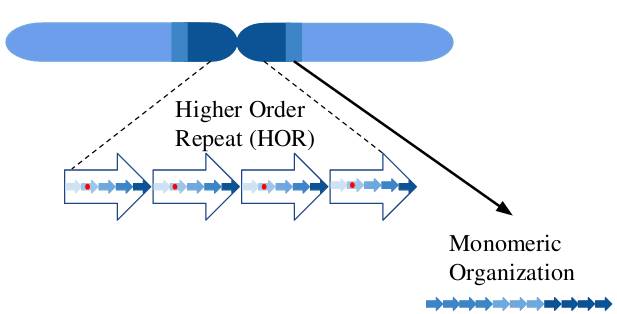
\includegraphics[height=5cm, width=10cm]{img/organization.png}
\caption{Organisation spatiale des $\alpha$-satellites. Une couleur correspond à un monomère d'une famille. Les points rouges représentent les sites de fixation à CENP-B.}
\end{figure}


\subsection{Le sujet de stage}
enchaîne sur l'étude chez les cerco, une autre étude de séquençage haut débit\\

-travaux précédents limités (expliquer pk). Les méthodes basées aur l'alignement et la phylogénie sont très limitées, le jeu de données étant trop grand. Les méthodes n'étaient pas objectives (quelles méthodes??). De plus, chez d'autres espèces de Primates, les informations sont trop dispersées et aucune comparaison interespèce n'a été faite. \\


L'équipe d'accueil de mon stage "ADN répété, Chromatine, Evolution" ou ARChE, a récemment développé une approche de séquençage haut débit, ciblée sur les séquences $\alpha$-satellites chez deux espèces de Cercopithèques. Une autre étude avec un grand nombre de séquences concerne le Gorille [Catacchio] avec l'utilisation de fragments relativement longs. 

L'objectif de ce stage est de comprendre la fonction des $\alpha$-satellites et leur mécanisme d'évolution. Je vais choisir plusieurs espèces de Primates. Je vais utiliser une méthode de classification automatisée améliorée du laboratoire [Florence Jornod] pour classer les séquences en familles.  Ce programme permet de traiter des centaines de milliers de séquences sans quelque soit le nombre de séquences ou la taille des familles. Je vais dans un premier temps appliquer cette technologies au données issues de ce séquençage. Ensuite, je vais étudier d'autres espèces. Puisque toutes les espèces sont étudiées par la  même méthode, une comparaison inter espèce est envisageable. 

%%%%%%%%%%%%%%%%%%%%%%%%%%%%%%%%%%%%%%%%%%%%%%%%%%%%%%%%%%%%%%%%%
%%%%%%%%%%%%%%%%%%%%%%M & M%%%%%%%%%%%%%%%%%%%%%%%%%%%%%%%%%%%%%%
%%%%%%%%%%%%%%%%%%%%%%%%%%%%%%%%%%%%%%%%%%%%%%%%%%%%%%%%%%%%%%%%% 
\section{Matériel et méthode}
\subsection{Choix des espèces}
Les critères de sélections dépendent de la disponibilité des séquences de qualité. Deux espèces du laboratoire, les \textit{Cercopithèques solatus} et \textit{pogonias}, et deux espèces proches, le \textit{Macaca fascicularis} et le \textit{Chlorocebus sabaeus}, sont choisies.  

%Les premières espèces choisies sont les \textit{Cercopithèques solatus} et \textit{pogonias}. L'équipe, ayant séquencé leur génome, donnent une description au préalable des $\alpha$-satellites. Je vais donc appliquer aux séquences issues des ces travaux notre méthode de classification automatisée puis comparer les familles acquises via ces deux approches.
 
%Le choix des espèces suivantes, le \textit{Macaca fascicularis} et le \textit{Chlorocebus sabaeus}, est fait selon la qualité des reads, obtenus par séquençage haut débit. En effet, les séquences doivent avoir une taille assez longue, soit au minimum 170 pb. Toutes ces espèces sont relativement proches, dans le but de faire des comparaisons inter-espèce par la suite.
 
\subsection{Méthode de classification}

Cette méthode [f.jornod] répartit des séquences $\alpha$-satellites en familles selon la similarité. La classification est hiérarchique dichotomique. Les séquences sont séparées en fonction de la fréquence des k-mers qui composent les séquences. Cette valeur k est déterminée à 5 à partir des études sur les \textit{Cercopithèques}. Elle décrit la diversité des séquences en optimisant l'usage de la mémoire. Une table de 5-mers est calculée pour toutes les séquences en début de programme.

La classification est suivie d'une double validation des sous-groupes. D'une part la taille du sous-groupe est vérifiée. La taille minimale d'une famille est fixée à 100. Si un groupe atteint 100 séquences, il n'est pas redivisé. D'autre part les deux groupes doivent être distincts. Pour cela le matepair est évalué. C'est la proportion de monomères ayant son plus proche voisin dans le même groupe. Des valeurs matepairs élevées indiquent des sous-groupes bien homogènes et séparés validant la classification tandis qu’un seuil matepair plus faible entraînera plus de classes. Si les matepairs sont au dessus d’un certain seuil, les deux sous-groupes sont ajoutés séparément à la file pour être potentiellement redivisés ultérieurement.En revanche, si au moins une des valeurs de matepair est au dessous de ce seuil, les sous-groupes seront considérés comme formant un seul groupe et le groupe initial est sauvegardé comme une famille unique. 

La séparation des séquences se fait de façon itérative en boucle. Chaque tour implique une analyse en composante principale (ACP), une classification hiérarchique et une analyse discriminante linéaire (LDA) si le jeu de données est conséquent. L'ACP est faite sur la table des k-mers pour réduire les dimensions du jeu de données en minimisant la perte d'information et obtenir des variables indépendantes utilisables pour la LDA. Le nombre de composantes est fixé à 1024. Ensuite des distances euclidiennes sont calculées entre toutes les paires de séquences dans l’espace défini par les M premières composantes de l’ACP. Puis la méthode de classification hiérarchique de Ward forme des classes de façon à minimiser l’inertie interclasse. Cependant, si le jeu de données dépasse 110 000 séquences, le calcul des distances devient pesant. La LDA entre alors en jeu. Cette méthode d'apprentissage utilise un sous-jeu de données formé par des séquences tirées aléatoirement. Le modèle construit est appliqué sur toutes les séquences.

%Ce programme, qui prend des séquence fasta en entrée, a été appliqué à des séquences humaines pour valider la méthodes.
%Le matepair correspond au nombre de séquences ayant la séquence la plus proche dans le même sous-groupes.

\subsection{Alignement, consensus et phylogénie}
%%%%%%%%%%%%%%%%%%%%%%%%%%%%%%%%%%%%%%%%%%%%%%%%%%%%%%%%%%%%%%%%%
%%%%%%%%%%%%%%%%%%%%%%%%%%%%%%%%%%%%%%%%%%%%%%%%%%%%%%%%%%%%%%%%%
%%%%%%%%%%%%%%%%%%%%%%%%%%%%%%%%%%%%%%%%%%%%%%%%%%%%%%%%%%%%%%%%%
\section{Résultat}
\section{Discussion}
\section{Conclusion}


%
%	\makeindex % index général
%   \newindex{env}{enx}{end}{Environnements}
%   \newindex{ext}{exx}{exd}{Extensions}
%   \newindex{cmm}{cmx}{cmd}{Commandes}
%	\newcommand{\commande}[1]
%   {\texttt{\textbackslash #1}}
%	\newcommand{\indexcmm}[1]
%   {\index[cmm]{#1@\commande{#1}}} % index d'une commande
% 
%
%
%
%Une citation\index{citation} hors paragraphe
%se met dans un environnement
%\emph{quote}\index[env]{quote}
%ou \emph{quotation}\index[env]{quotation}
% 
%L'extension \emph{array}\index[ext]{array}
%fournit les commandes
%\commande{raggedleft}\indexcmm{raggedleft}
%et \commande{raggedright}\indexcmm{raggedright}.
% 
%\printindex % index général
%\printindex[env]
%\printindex[ext]
%\printindex[cmm]

\end{document}
%
%%HELP: http://lataix-sebastien.developpez.com/tutoriels/latex/memoire-de-fin-d-etude/#LII-C